\documentclass{article}

\usepackage{amsmath}
\usepackage{graphicx}
\usepackage{listings}
\usepackage{color}

\definecolor{dkgreen}{rgb}{0,0.6,0}
\definecolor{gray}{rgb}{0.5,0.5,0.5}
\definecolor{mauve}{rgb}{0.58,0,0.82}

\lstset{frame=tb,
    language=Python,
    aboveskip=3mm,
    belowskip=3mm,
    showstringspaces=false,
    columns=flexible,
    basicstyle={\small\ttfamily},
    numbers=none,
    numberstyle=\tiny\color{gray},
    keywordstyle=\color{blue},
    commentstyle=\color{dkgreen},
    stringstyle=\color{mauve},
    breaklines=true,
    breakatwhitespace=true,
    tabsize=3
}

\title{Assignment 2: Simple TTS using a vocoder-like method}
\author{Aleksandr Jan Smoliakov}
\date{2024--11--05}

\begin{document}

\maketitle

\section{Introduction}

In this project, we aim to implement a simple vocoder pipeline for speech synthesis by converting a waveform into a Mel spectrogram and reconstructing it back into a waveform. Vocoders are essential in text-to-speech (TTS) applications as they provide a mechanism to synthesize speech from spectral representations, preserving critical acoustic information. This approach will allow us to understand the basics of audio reconstruction and assess the quality of synthesized audio. The task will involve both subjective (Mean Opinion Score, MOS) and objective (Perceptual Evaluation of Speech Quality, PESQ) evaluations, providing insight into how accurately the vocoder method can reproduce pitch and timbre.

\section{Methodology}

This section outlines steps involved in the vocoder pipeline, covering the process of generating a Mel spectrogram from an audio waveform and reconstructing it back into a waveform.

\subsection{Waveform to Mel Spectrogram Conversion}

The first step in the pipeline is to convert the input waveform into a Mel spectrogram. A Mel spectrogram represents the time-varying frequency content of the audio, scaled according to the Mel scale, which approximates the way humans perceive pitch.

\subsubsection{Short-Time Fourier Transform (STFT)}

To generate a Mel spectrogram, we start by applying the Short-Time Fourier Transform (STFT) to the waveform. The STFT breaks down the audio signal into short overlapping segments along the time axis, computing a Fourier Transform for each segment. This results in a time-frequency representation of the audio, where each time frame contains frequency information about a short segment of the signal. The STFT is parameterized by the window size (the length of each segment) and hop length (the overlap between segments). In this task, a window size of 1024 samples and hop length of 256 samples. At 16 kHz, this corresponds to a window size of 64 ms and a hop length of 16 ms.

Thus, if initially 1s of audio signal sampled at 16 kHz is provided, the 1D waveform of length 16000 will be transformed into a 2D matrix of shape (513, 64) where 513 is the number of frequency bins and 64 is the number of time frames.

\subsubsection{Mel Scale Transformation}

After obtaining the STFT spectrogram, we map the frequency axis to the Mel scale. The Mel scale is a perceptual scale of frequency (similar to logarithmic) that is more aligned with how humans hear sound. Frequencies are converted to the Mel scale by applying a set of overlapping triangular filter banks that emphasize lower frequencies more heavily than higher ones, since humans are more sensitive to lower frequencies. This transformation results in a Mel spectrogram, which is a compressed, perceptually meaningful representation of the signal. In this task, we use 96 Mel filters to capture the frequency content of the audio signal.

Thus, 1s of audio signal sampled at 16 kHz will be transformed into a matrix of shape (96, 64) where 96 is the number of Mel frequency bins and 64 is the number of time frames.

\subsection{Waveform Reconstruction with Griffin-Lim Algorithm}

To reconstruct the waveform from the Mel spectrogram, we utilize the Griffin-Lim algorithm. It is an iterative algorithm that estimates the missing phase information from magnitude spectrogram data. The signal is converted back into a time-domain signal. Griffin-Lim is commonly used in vocoder setups due to its effectiveness in producing intelligible audio with limited phase data, though it is known to introduce artifacts.

After this step, the Mel spectrogram is converted back into a waveform, and 1s of audio is again represented as a 1D waveform of length 16000.

\subsubsection{Phase Estimation with Griffin-Lim}

Griffin-Lim algorithm iteratively refines an initial guess of the phase by minimizing the error between the reconstructed spectrogram and the original magnitude spectrogram. At each iteration, a phase estimate is applied to the magnitude spectrogram, and the inverse STFT is performed to produce a time-domain signal. This signal is then converted back to a spectrogram to update the phase estimate. The iterative process continues until the estimated phase reaches a predefined number of iterations (60 in our project). While effective, Griffin-Lim is known to produce artifacts, such as metallic resonance, due to imperfect phase reconstruction.

\subsection{Pitch (F0) and PESQ Evaluation}

Evaluation of the reconstructed waveform can assess the effectiveness of the vocoder pipeline. Along with F0 evalation, we will employ one objective and one subjective metric for a comprehensive analysis of quality.

\subsubsection{Pitch (F0) Analysis}

Pitch (F0) represents the fundamental frequency of a sound and is essential in preserving the naturalness and expressiveness of speech. We will calculate the F0 contour of both the original and synthesized waveforms to assess pitch accuracy. The F0 contour provides insights into how well the reconstructed waveform captures the tonal fluctuations and intonation of the original performance, which is particularly relevant in speech and music applications.

\subsubsection{Perceptual Evaluation of Speech Quality (PESQ)}

For objective evaluation, we compute the PESQ (Perceptual Evaluation of Speech Quality) score of the reconstructed audio. Additionally, we analyze the pitch (F0) contour of both the original and synthesized signals, using the pitch accuracy as a measure of quality. This analysis will help identify any discrepancies in the reproduced pitch and assess the degree to which the original vocal expression is retained.

PESQ compares the original and reconstructed waveforms and provides a score that correlates with human perceptions of audio quality. This evaluation function returns a score between -0.5 and 4.5, with higher scores indicating better quality. A score of 4.5 represents perfect quality, while a score of 1.0 is considered acceptable for most applications.

\subsubsection{Mean Opinion Score (MOS)}

For subjective evaluation, we will assign MOS (Mean Opinion Score) on a scale of 1 to 5. Essentially, what this means is that we will rate the quality of the reconstructed audio based on how it sounds to us. This will provide a qualitative assessment of the overall quality of the synthesized audio, focusing on aspects such as pitch accuracy, timbre, and overall naturalness.

\section{Analysis and Results}

In this section, we apply the vocoder pipeline to a 25-second excerpt from Luciano Pavarotti's performance of \textit{Nessun Dorma} from Puccini's opera \textit{Turandot}. The audio is sampled at 16 kHz. We visualize and evaluate various aspects of the original and reconstructed waveforms.

\begin{figure}[!htbp]
    \centering
    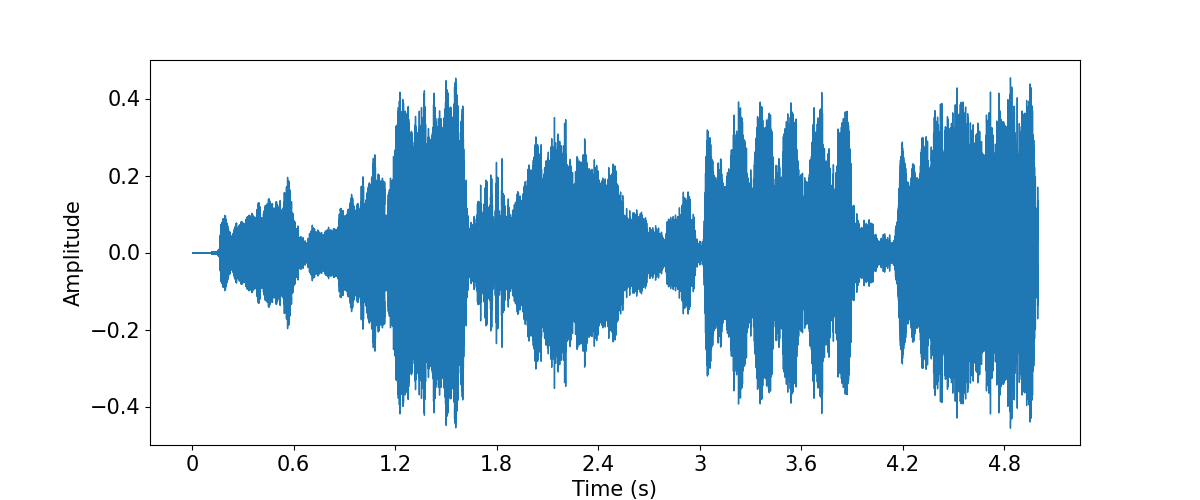
\includegraphics[width=\textwidth]{data/plots/nessun_dorma_trimmed_original_waveform.png}
    \caption{Original waveform of the audio file, first 5 seconds.}
    \label{fig:original_waveform}
\end{figure}

Figure~\ref{fig:original_waveform} shows the original waveform of the audio file, focusing on the first 5 seconds for clarity.

\begin{figure}[!htbp]
    \centering
    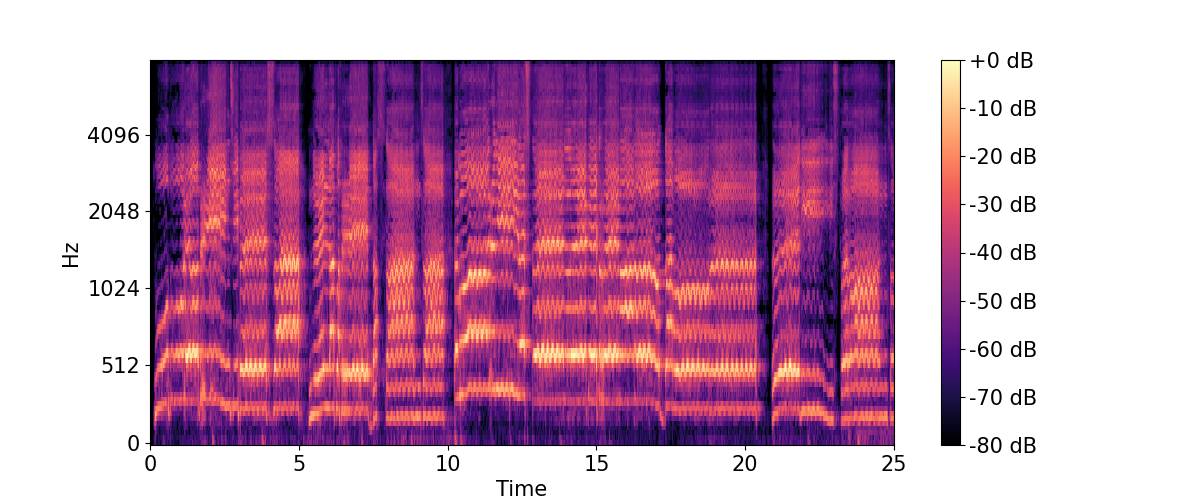
\includegraphics[width=\textwidth]{data/plots/nessun_dorma_trimmed_mel_spectrogram.png}
    \caption{Mel spectrogram of the audio file.}
    \label{fig:mel_spectrogram}
\end{figure}

The Mel spectrogram of the audio file is shown in Figure~\ref{fig:mel_spectrogram}, illustrating the energy distribution across time and frequency.

\begin{figure}[!htbp]
    \centering
    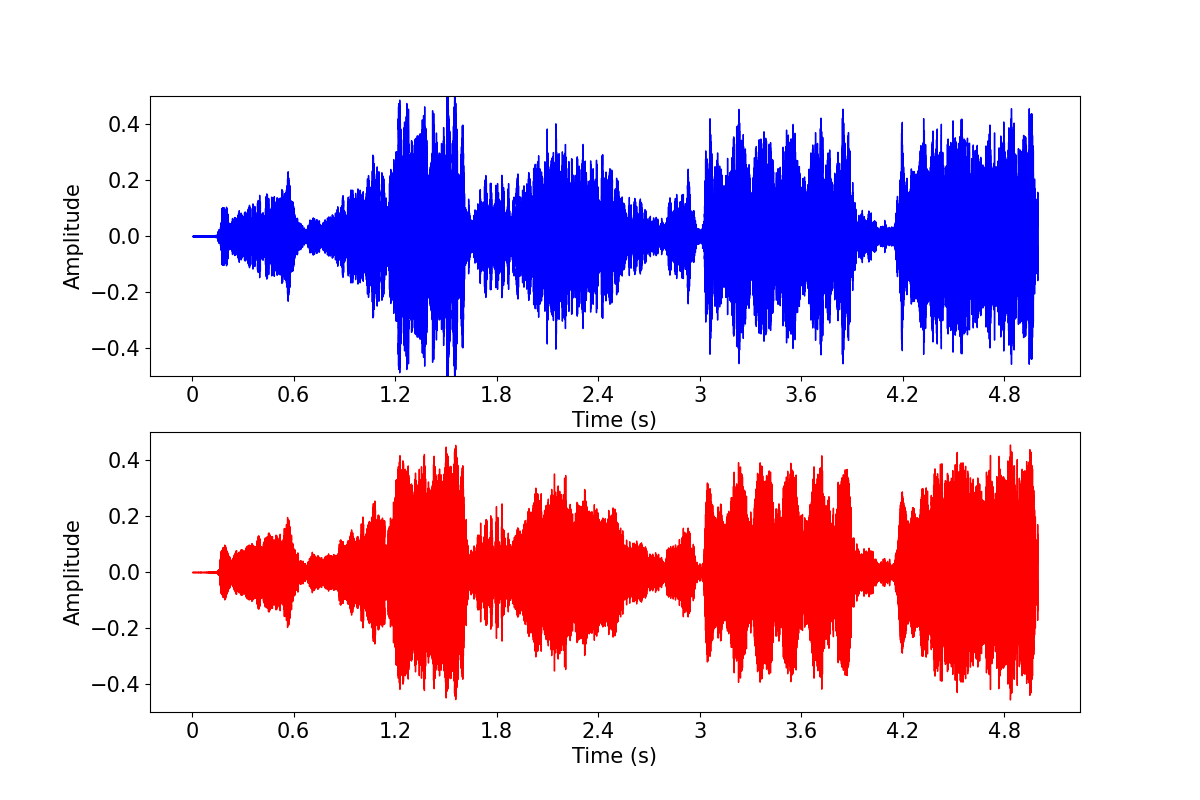
\includegraphics[width=\textwidth]{data/plots/nessun_dorma_trimmed_original_vs_reconstructed_waveform.png}
    \caption{Comparison between the original (top) and reconstructed (bottom) waveforms.}
    \label{fig:original_vs_reconstructed_waveform}
\end{figure}

Figure~\ref{fig:original_vs_reconstructed_waveform} shows a comparison between the original and reconstructed waveforms.

\begin{figure}[!htbp]
    \centering
    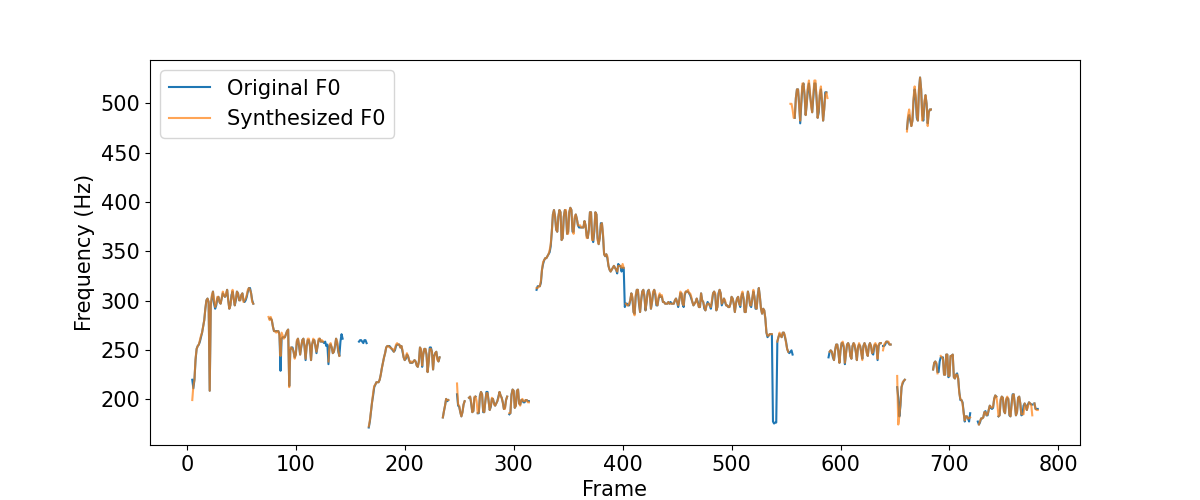
\includegraphics[width=\textwidth]{data/plots/nessun_dorma_trimmed_f0_contour.png}
    \caption{Pitch contour (F0) comparison between the original and reconstructed waveforms.}
    \label{fig:f0_contour}
\end{figure}

Figure~\ref{fig:f0_contour} compares the pitch (F0) contour of the original and reconstructed waveforms, showing how accurately pitch has been preserved.

\begin{figure}[!htbp]
    \centering
    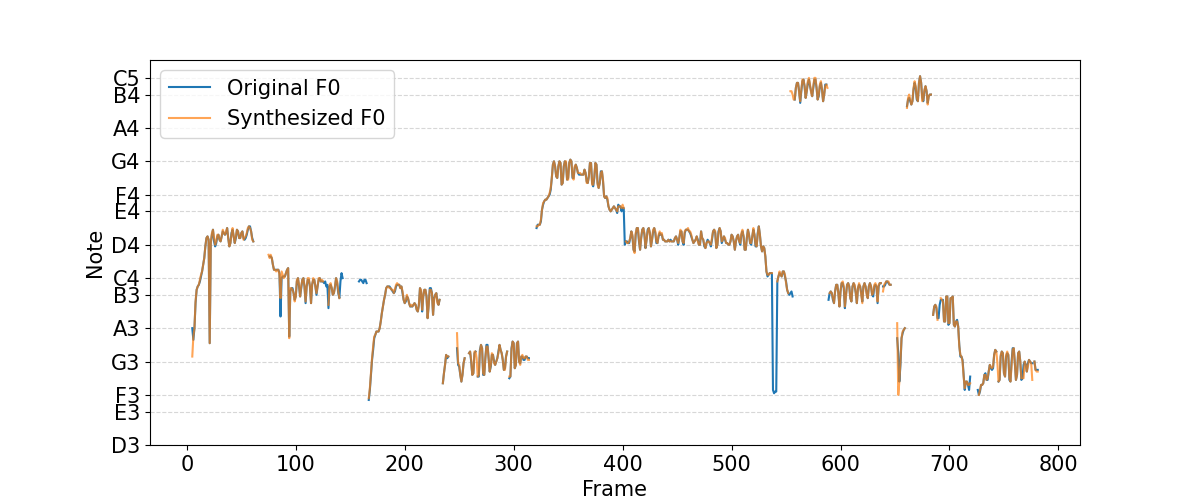
\includegraphics[width=\textwidth]{data/plots/nessun_dorma_trimmed_f0_contour_notes.png}
    \caption{Pitch contour (F0) comparison between the original and reconstructed waveforms with note names displayed.}
    \label{fig:f0_contour_notes}
\end{figure}

The PESQ score for the reconstructed waveform is 2.54, indicating a fair level of quality in the reconstruction. Subjective listening confirms that while the pitch and general structure are preserved, there are noticeable timbre distortions.

\section{Conclusions}

Overall, subjectively the reconstructed waveform sounds very similar to the original waveform, capturing the general characteristics of the aria. Personally I would rate the quality of the reconstructed audio as 3 out of 5. I cannot hear significant pitch distortions, and the characteristic vibrato of Pavarotti's voice is preserved in the reconstructed waveform. However, there are noticeable timbre distortions present in the reconstructed waveform, with strange metallic resonances that are not present in the original one.

These findings align with the computed PESQ score of 2.54, which indicates fair quality. The pitch (F0) contour comparison shows that the reconstructed waveform captures the pitch variations of the original performance very well.

These distortions may be attributed to limitations in the Griffin-Lim algorithm's phase estimation. Artifacts of this nature are common in spectrogram-based synthesis due to phase errors and the limited amount of information available in the Mel spectrogram.

Modern vocoders based on neural networks such as HiFi-GAN and WaveNet have shown superior quality due to their ability to model the time-domain waveform directly or to learn richer spectral representations. These models can better capture subtleties in phase and timbre, avoiding artifacts commonly observed in Griffin-Lim reconstructions. However, the simplicity and interpretability of the vocoder pipeline presented here make it a valuable starting point for understanding the basics of speech synthesis.

All in all, this project successfully demonstrates a simple vocoder pipeline, converting a waveform into a Mel spectrogram and back. While the reconstructed waveform retains key elements of the original, limitations in phase reconstruction and timbre accuracy suggest room for improvement. Modern neural vocoders offer promising alternatives that address these issues, producing higher-quality results.

\newpage

\section{Appendix 1: Source Code}

Source code used in this solution is presented below. The code is written in Python 3.11 and uses the following libraries: \texttt{librosa}, \texttt{numpy}, \texttt{matplotlib}, \texttt{soundfile}, \texttt{pesq}.

\begin{lstlisting}
import argparse
import logging
import librosa
import librosa.display
import numpy as np
import matplotlib.pyplot as plt
import soundfile as sf
from pathlib import Path
from pesq import pesq

logging.basicConfig(level=logging.INFO)

plt.rcParams.update({"font.size": 15})

# constants
INPUT_DIR = Path("data/input")
OUTPUT_DIR = Path("data/output")
PLOT_DIR = Path("data/plots")
NOTE_NAMES = (
    ["D3", "E3", "F3", "G3", "A3", "B3"]
    + ["C4", "D4", "E4", "F4", "G4", "A4", "B4", "C5"]
)


parser = argparse.ArgumentParser(
    description="Convert an audio file to a Mel spectrogram and back to a waveform.",
)
parser.add_argument(
    "--n_fft",
    type=int,
    default=1024,
    help="Number of samples in each window of the STFT.",
)
parser.add_argument(
    "--hop_length",
    type=int,
    default=256,
    help="Number of samples between successive frames.",
)
parser.add_argument(
    "--n_mels",
    type=int,
    default=96,
    help="Number of Mel bands to generate.",
)


def draw_plots(
    waveform: np.ndarray,
    reconstructed_waveform: np.ndarray,
    mel_spectrogram: np.ndarray,
    filename_stem: str,
    sample_rate: int,
    hop_length: int,
) -> None:
    # original waveform
    plt.figure(figsize=(12, 5))
    librosa.display.waveshow(
        waveform[: 5 * sample_rate],
        sr=sample_rate,
    )
    plt.xlabel("Time (s)")
    plt.ylabel("Amplitude")
    plt.ylim(-0.5, 0.5)
    plt.savefig(PLOT_DIR / f"{filename_stem}_original_waveform.png")

    # original vs reconstructed waveform
    plt.figure(figsize=(12, 8))
    plt.subplot(2, 1, 1)
    librosa.display.waveshow(
        reconstructed_waveform[: 5 * sample_rate],
        sr=sample_rate,
        color="b",
    )
    plt.xlabel("Time (s)")
    plt.ylabel("Amplitude")
    plt.ylim(-0.5, 0.5)

    plt.subplot(2, 1, 2)
    librosa.display.waveshow(
        waveform[: 5 * sample_rate],
        sr=sample_rate,
        color="r",
    )
    plt.xlabel("Time (s)")
    plt.ylabel("Amplitude")
    plt.ylim(-0.5, 0.5)
    plt.savefig(PLOT_DIR / f"{filename_stem}_original_vs_reconstructed_waveform.png")

    # convert to log scale (dB) for better visualization
    log_mel_spectrogram = librosa.power_to_db(mel_spectrogram, ref=np.max)

    # Mel spectrogram of the original waveform
    plt.figure(figsize=(12, 5))
    librosa.display.specshow(
        log_mel_spectrogram,
        sr=sample_rate,
        hop_length=hop_length,
        x_axis="time",
        y_axis="mel",
    )
    plt.colorbar(format="%+2.0f dB")
    plt.savefig(PLOT_DIR / f"{filename_stem}_mel_spectrogram.png")

    # evaluate pitch (F0 contour) of the synthesized speech
    f0_original, _, _ = librosa.pyin(
        waveform,
        fmin=librosa.note_to_hz("C2"),
        fmax=librosa.note_to_hz("C7"),
        sr=sample_rate,
    )
    f0_synthesized, _, _ = librosa.pyin(
        reconstructed_waveform,
        fmin=librosa.note_to_hz("C2"),
        fmax=librosa.note_to_hz("C7"),
        sr=sample_rate,
    )

    # F0 contour (pitch variation over time)
    plt.figure(figsize=(12, 5))
    plt.plot(f0_original, label="Original F0")
    plt.plot(f0_synthesized, label="Synthesized F0", alpha=0.7)
    plt.xlabel("Frame")
    plt.ylabel("Frequency (Hz)")
    plt.legend()
    plt.savefig(PLOT_DIR / f"{filename_stem}_f0_contour.png")

    # F0 contour (pitch variation over time) - display note names, log scale
    plt.figure(figsize=(12, 5))
    plt.plot(f0_original, label="Original F0")
    plt.plot(f0_synthesized, label="Synthesized F0", alpha=0.7)
    plt.xlabel("Frame")
    plt.ylabel("Note")
    plt.legend()
    plt.yscale("log")
    plt.yticks([librosa.note_to_hz(note) for note in NOTE_NAMES], NOTE_NAMES)
    plt.grid(which="both", axis="y", linestyle="--", alpha=0.5)
    plt.minorticks_off()
    plt.savefig(PLOT_DIR / f"{filename_stem}_f0_contour_notes.png")


def process_audio_file(
    filename: Path,
    n_fft: int,
    hop_length: int,
    n_mels: int,
) -> None:
    # load an audio file
    waveform, sample_rate = librosa.load(filename, sr=None)
    logging.info(f"Duration: {len(waveform) / sample_rate:.2f} seconds")
    logging.info(f"Sample rate: {sample_rate}")

    assert sample_rate in [8000, 16000], "PESQ only supports 8kHz and 16kHz."

    # compute the STFT (magnitude)
    stft = np.abs(librosa.stft(waveform, n_fft=n_fft, hop_length=hop_length))

    # generate a Mel filter bank
    mel_filter_bank = librosa.filters.mel(sr=sample_rate, n_fft=n_fft, n_mels=n_mels)

    # apply the Mel filter bank to the power spectrogram
    mel_spectrogram = np.dot(mel_filter_bank, stft**2)

    # convert Mel spectrogram back to STFT magnitude spectrogram
    stft_magnitude = librosa.feature.inverse.mel_to_stft(
        mel_spectrogram,
        sr=sample_rate,
        n_fft=n_fft,
        power=2,
    )

    # reconstruct waveform using Griffin-Lim
    reconstructed_waveform = librosa.griffinlim(
        stft_magnitude,
        hop_length=hop_length,
        n_fft=n_fft,
        n_iter=60,
    )

    # save the reconstructed waveform as a .wav file
    reconstructed_filename = OUTPUT_DIR / filename.name
    sf.write(reconstructed_filename, reconstructed_waveform, sample_rate)

    # perform PESQ evaluation
    pesq_score = pesq(sample_rate, waveform, reconstructed_waveform)
    logging.info(f"PESQ score: {pesq_score:.2f}")

    # visualize the results
    draw_plots(
        waveform=waveform,
        reconstructed_waveform=reconstructed_waveform,
        mel_spectrogram=mel_spectrogram,
        filename_stem=filename.stem,
        sample_rate=sample_rate,
        hop_length=hop_length,
    )


if __name__ == "__main__":
    args = parser.parse_args()

    # create directories if they don't exist
    INPUT_DIR.mkdir(parents=True, exist_ok=True)
    OUTPUT_DIR.mkdir(parents=True, exist_ok=True)
    PLOT_DIR.mkdir(parents=True, exist_ok=True)

    filenames = list(INPUT_DIR.glob("*.wav"))

    # validate input files
    assert len(filenames) > 0, "No input files provided."

    # process each audio file
    for filename in filenames:
        logging.info(f"Processing {filename}")
        process_audio_file(
            filename,
            n_fft=args.n_fft,
            hop_length=args.hop_length,
            n_mels=args.n_mels,
        )
        logging.info("\n")
\end{lstlisting}

\end{document}
